
\documentclass[xcolor={dvipsnames}]{beamer}
\usepackage{amsmath,amsfonts,amssymb,pxfonts,eulervm,xspace}
\usepackage{graphicx}
 \usepackage{multimedia}
\usepackage{media9}

\graphicspath{{./figures/}}
\usetheme{ccnycrest}


\newenvironment{changemargin}[2]{%
\begin{list}{}{%
\setlength{\topsep}{0pt}%
\setlength{\leftmargin}{#1}%
\setlength{\rightmargin}{#2}%
\setlength{\listparindent}{\parindent}%
\setlength{\itemindent}{\parindent}%
\setlength{\parsep}{\parskip}%
}%
\item[]}{\end{list}}

\begin{document}

\title{ CS102: Data Types}
\author{Hannah Aizenman}
\date{haizenm00@ccny.cuny.edu}


\begin{frame}
	\titlepage
\end{frame}

\begin{frame}
	\begin{center}
		Information is packaged in all sorts of ways...
	\end{center}
\end{frame}

\begin{frame}{Text}
	\begin{quote}
	 ...it became instantly clear why inundation was a serious problem ... more than 80\% of the data is missing as measured by 100*isNAN/datapoints...
	\end{quote}
\end{frame}

\begin{frame}{Numbers}
	\begin{figure}
			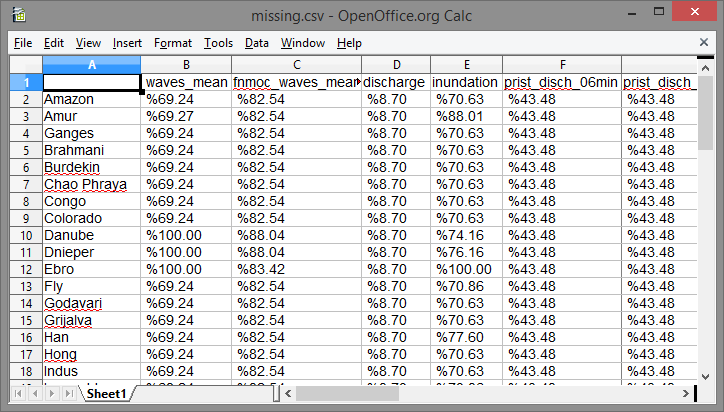
\includegraphics[width=1\textwidth]{numbers}
	\end{figure}
\end{frame}

\begin{frame}{Pictures}
	\begin{figure}
		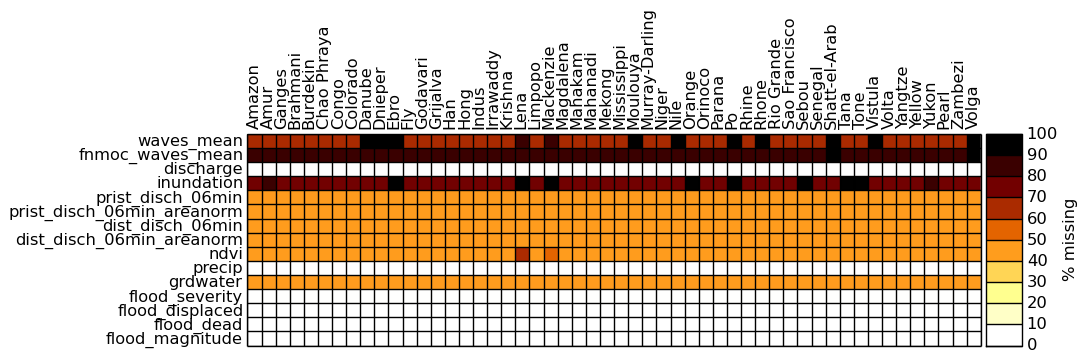
\includegraphics[width=1\textwidth]{missing}
	\end{figure}
\end{frame}

\begin{frame}
	\begin{center}
	...so how do computers represent information?
	\end{center}
\end{frame}

\begin{frame}{Binary}
	\begin{itemize}
		\item computers store information using digital components
		\pause
		\item these components only have on/off states
		\pause
		\item each component can store one value
		\pause
		\item these values are called bits
		\pause
		\item early computers stored the data using switches
	\end{itemize}
\end{frame}

\begin{frame}{Binary 0}
	\begin{figure}
		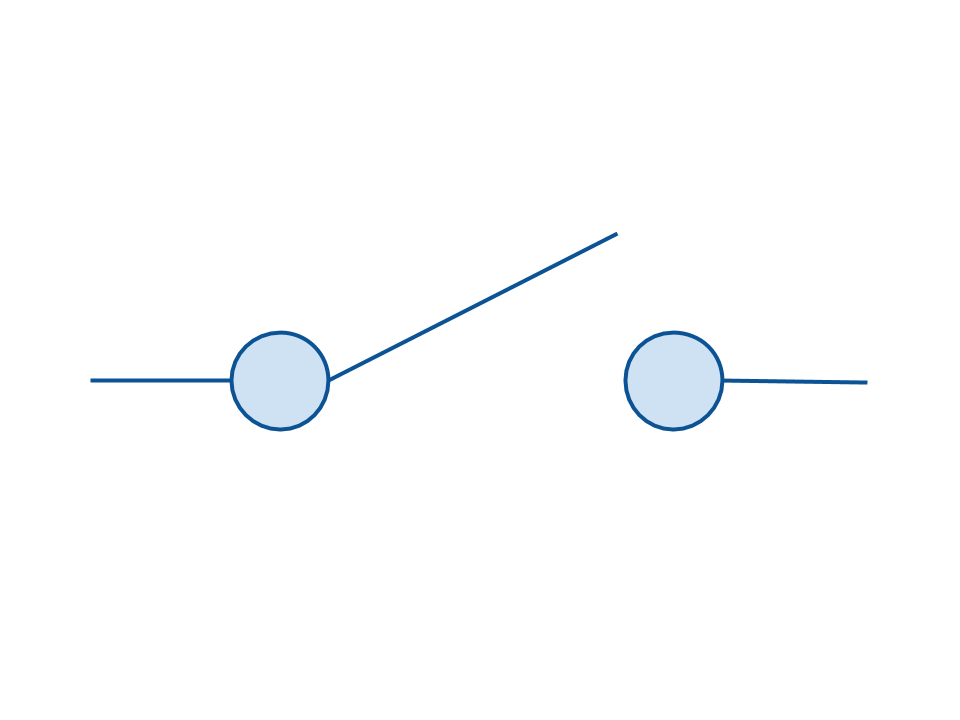
\includegraphics[trim =3cm 6cm 3cm 6cm, clip=true, width=1\textwidth]{open}
		\caption{An open switch or low voltage is a binary 0}
	\end{figure}
\end{frame}

\begin{frame}{Binary 1}
	\begin{figure}	
		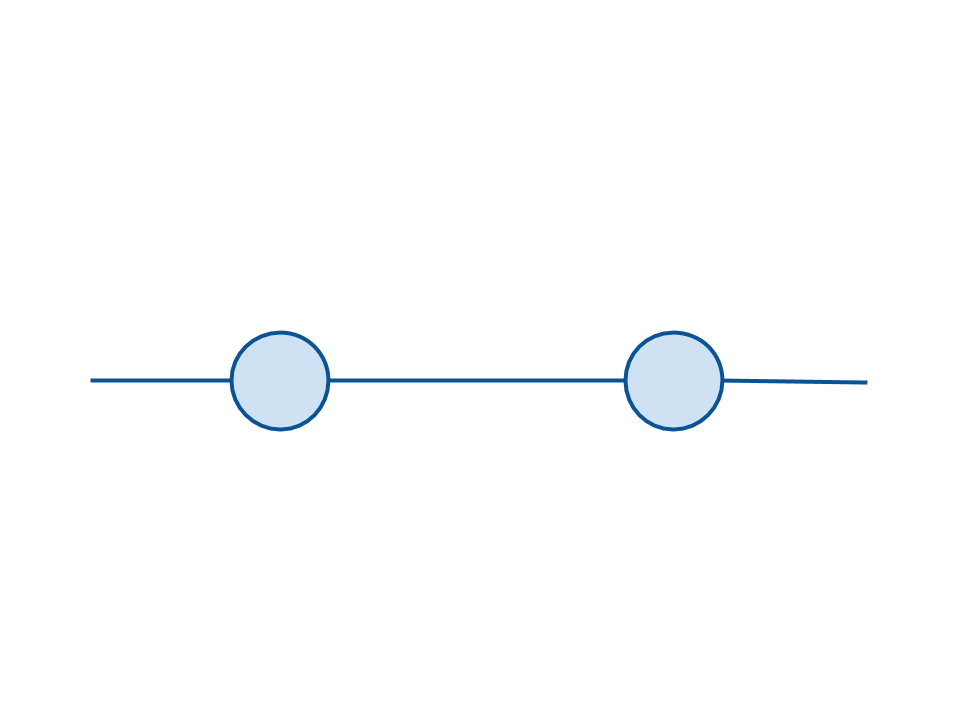
\includegraphics[trim =3cm 6cm 3cm 6cm, clip=true, width=1\textwidth]{close}
		\caption{A closed switch or high voltage is a binary 1}
	\end{figure}
\end{frame}

\begin{frame}{Counting in Binary}
	\begin{center}
	\begin{tabular}{c | l}
		Binary & \\
		\hline
		0 & start\\
		1 & next \\
		??? & there's no 2! \\
	\end{tabular}
	\end{center}
\end{frame}


\begin{frame}{Counting in Decimal}
	\begin{center}
	\begin{tabular}{c | l}
		Binary & \\
		\hline
		0 & start \\
		1, 2, ...7, 8 & \\
		9 & last decimal digit \\
		10 & go back to 0, but put a 1 in the 10s place
	\end{tabular}
	\end{center}
\end{frame}

\begin{frame}{Counting in Binary}
	\begin{center}
	\begin{tabular}{c | l}
		Binary & \\
		\hline
		0 & start\\
		1 & next \\
		10 & back at 0, but add a 1 in the next place\\
		11 & ...
	\end{tabular}
	\end{center}
\end{frame}

\begin{frame}{Binary: Whole Number}
	\begin{figure}
		\href{http://www.wikihow.com/Convert-from-Binary-to-Decimal}{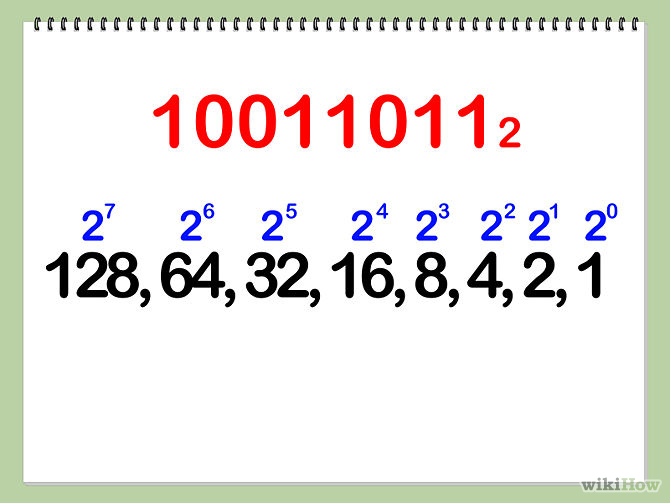
\includegraphics[width=1\textwidth]{binary_decimal}}
	\end{figure}
\end{frame}

\begin{frame}{Binary: Whole Number}
	\begin{figure}
		\href{http://www.wikihow.com/Convert-from-Binary-to-Decimal}{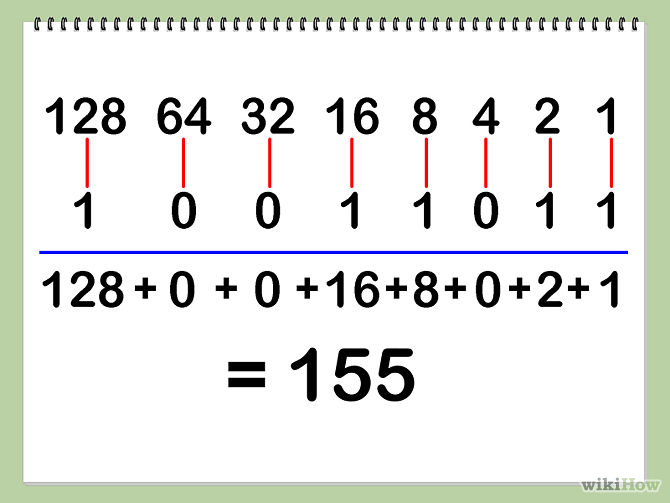
\includegraphics[width=1\textwidth]{binary_decimal_2}}
	\end{figure}
\end{frame}

\begin{frame}{Binary: Decimal Number}
	\begin{figure}
		\href{http://www.mathsisfun.com/binary-number-system.html}{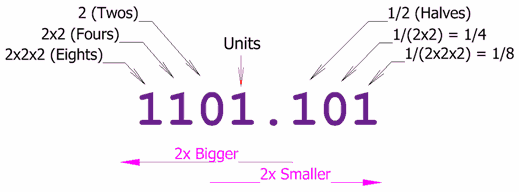
\includegraphics[width=1\textwidth]{binary_number}}
	\end{figure}
\end{frame}

\begin{frame}{Binary: Floating Point}
	\begin{figure}
	\href{http://www.teach-ict.com/as_as_computing/ocr/H447/F453/3_3_4/floating_point/miniweb/pg6.htm}{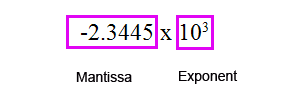
\includegraphics[width=1\textwidth]{floatingpoint}}\\			\href{http://www.teach-ict.com/as_as_computing/ocr/H447/F453/3_3_4/floating_point/miniweb/pg6.htm}{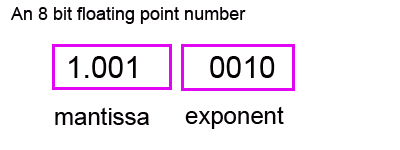
\includegraphics[width=1\textwidth]{mantissa}}
	\end{figure}
\end{frame}

\begin{frame}{Binary: Letter or Symbol (ASCII)}
	\begin{figure}
		\href{https://commons.wikimedia.org/wiki/File:ASCII-Table.svg}{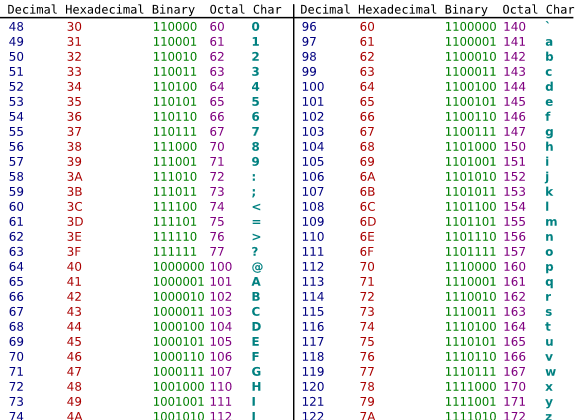
\includegraphics[width=1\textwidth]{ascii}}
	\end{figure}
\end{frame}

\begin{frame}{Datatypes}
	\begin{itemize}
		\item compilers can't tell symbols and the different types of numbers apart
			\pause
		\item \textbf{datatypes} tell the compiler what it's working with
			\pause
		\item built-in datatypes are called \textbf{primitives}:
			\pause
			\begin{description}
				\item [integer] whole number
				\item [double] decimal number
				\item [float] floating point number
				\item [character] letter or symbol
				\item [bool] true, false
			\end{description}
	\end{itemize}
\end{frame}

\begin{frame}{Variables}
	Variables are used to store information for later use. 
	\begin{figure}
		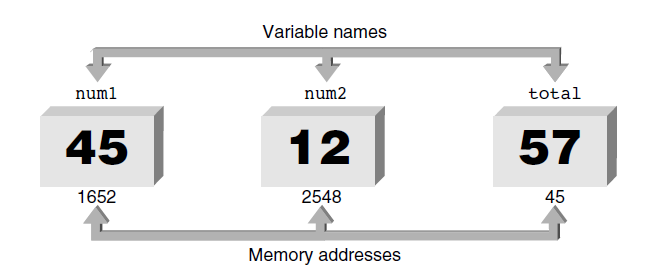
\includegraphics[width=1\textwidth]{variable}
		\caption{Variables consist of a name, type, and value}
	\end{figure}
\end{frame}

\begin{frame}{Variables}
	\begin{description}
		\item[name] how the variable is referred to throughout the code
		\pause
		\item[type] the datatype of the information the variable stores
		\pause
		\item[value] the information the variable stores
	\end{description}
\end{frame}

\begin{frame}{Variable name}
	There are a few rules for variable names(identified)
	\begin{itemize}
		\pause
		\item First character has to be a letter or underscore
			\begin{description}
				\item[good] hello, \textunderscore hello
				\item[bad] 1hello, @hello
			\end{description}
		\pause
		\item Must be composed of letters, digits, and underscores
			\begin{description}
				\item[good] hello1, he1llo, he\textunderscore llo
				\item[bad] h*ello, he llo
			\end{description}
		\pause
		\item Can't be part of the language
				\begin{description}
				\item[good] hello, goodbye, world
				\item[bad] int, using, return
			\end{description}
		\pause
		\item Can't have more than 1024 characters 
	\end{itemize}	
\end{frame}

\begin{frame}{Declaration Statement}
	\begin{block}{How they work:}
		\begin{itemize}
			\item identifies the variable \textbf{name}
			\item specifies the variable \textbf{type}
		\end{itemize}
	\end{block}
	\pause
	\begin{block}{How they're written:}
		\begin{center}
			\textcolor{DarkOrchid}{\textbf{type}} \textit{name};\\
			\pause
			\textcolor{DarkOrchid}{\textbf{type}} \textit{name1}, \textit{name2}, \textit{name3}, ...;
		\end{center}
	\end{block}
\end{frame}

\begin{frame}{Declaration: integer}
	\begin{itemize}
		\item \textcolor{DarkOrchid}{\textbf{int}} \textit{voltage};
		\item \textcolor{DarkOrchid}{\textbf{int}} \textit{power}, \textit{resistance};
	\end{itemize}
\end{frame}

\begin{frame}{Declaration: double}
	\begin{itemize}
		\item \textcolor{DarkOrchid}{\textbf{double}} \textit{temperature};
		\item \textcolor{DarkOrchid}{\textbf{double}} \textit{pressure}, \textit{wind};
	\end{itemize}
\end{frame}

\begin{frame}{Declaration: float}
	\begin{itemize}
		\item \textcolor{DarkOrchid}{\textbf{float}} \textit{acceleration};
		\item \textcolor{DarkOrchid}{\textbf{float}} \textit{gravity}, \textit{velocity};
	\end{itemize}
\end{frame}

\begin{frame}{Declaration: character}
	\begin{itemize}
		\item \textcolor{DarkOrchid}{\textbf{char}} \textit{no\textunderscore quit};
		\item \textcolor{DarkOrchid}{\textbf{char}} \textit{no\textunderscore quit}, \textit{quit};
	\end{itemize}
\end{frame}

\end{document}

